\chapter{Memoria virtuale}

\section{Introduzione}
I metodi di gestione della Memoria Primaria (MP) cercano di mantenere in RAM il maggior numero possibile di processi per aumentare il livello di multiprogrammazione. Tuttavia, per una data quantità di RAM disponibile, il numero di processi che possono risiedere in MP dipende dalla loro dimensione.

\dfn{Memoria Virtuale (MV)}{
La \emph{Memoria Virtuale (MV)} è un insieme di tecniche che permette l'esecuzione di processi in cui codice e/o dati non sono completamente caricati in Memoria Primaria. La MV funziona poiché i programmi non necessitano di essere interamente presenti in MP per poter essere eseguiti. 
}

\ex{Esempi di utilizzo della Memoria Virtuale}{
- Il codice per la gestione delle condizioni di errore potrebbe non essere mai usato durante l’esecuzione di un programma.
- Array, liste e tabelle sono spesso dichiarate di dimensioni superiori a quanto effettivamente richiesto.
- Alcune opzioni di programma sono raramente utilizzate.
- Le librerie dinamiche vengono caricate in RAM solo se e quando effettivamente richieste.
}

L’idea alla base della Memoria Virtuale è la seguente:
\begin{itemize}
    \item Carichiamo in MP solo le parti di un programma che devono effettivamente essere eseguite e solo quando è necessario.
    \item Carichiamo in MP solo la porzione di strutture dati che sono utilizzate in una determinata fase di esecuzione.
\end{itemize}

\clm{Vantaggi della Memoria Virtuale}{}{
La Memoria Virtuale permette di eseguire programmi che superano la dimensione della MP. Formalmente:
\begin{itemize}
    \item È possibile eseguire un processo che utilizza uno spazio di indirizzamento logico superiore allo spazio fisico disponibile.
    \item È possibile avere in esecuzione contemporaneamente più processi che, sommati, occupano più spazio della MP disponibile.
    \item Ne consegue un aumento della multiprogrammazione e quindi del \emph{throughput} della CPU.
    \item I programmi possono iniziare l’esecuzione più velocemente, poiché non è necessario caricarli interamente in memoria primaria.
\end{itemize}
}

Naturalmente, vi sono anche degli \emph{inconvenienti} legati all'uso della Memoria Virtuale:
\begin{itemize}
    \item Si genera un aumento del traffico tra la RAM e l’hard disk.
    \item L'esecuzione di un singolo programma potrebbe richiedere più tempo rispetto a uno scenario senza MV.
    \item In situazioni particolari, le prestazioni complessive del sistema possono degradare drasticamente, fenomeno noto come \emph{thrashing}.
\end{itemize}

\section{Paginazione su richiesta (Demand Paging)}
L'idea di base della Memoria Virtuale è quella di \emph{portare una pagina in MP solo nel momento del primo indirizzamento di una locazione} (un dato, un'istruzione) appartenente alla pagina stessa.
Quando la CPU esegue un'istruzione che indirizza una locazione di RAM in una pagina diversa da quella contenente l'istruzione in esecuzione, e la pagina non è in MP, si dice che il processo ha generato un \emph{page fault}. In questo caso, il Sistema Operativo (SO) deve:
\begin{enumerate}
    \item sospendere il processo,
    \item portare in memoria la pagina mancante,
    \item una volta disponibile, riprendere l'esecuzione del processo dal punto in cui era stato interrotto.
\end{enumerate}
\subsection*{Passaggi per la gestione del page fault}
Più in dettaglio, quando manca la pagina riferita:
\begin{itemize}
    \item Il processo viene tolto dalla CPU e messo in uno stato di \emph{waiting for page}.
    \item Un modulo del SO detto \emph{pager} inizia il caricamento della pagina mancante dalla Memoria Secondaria (MS) in un frame libero della Memoria Primaria (MP).
    \item Nel frattempo, la CPU viene assegnata a un altro processo.
    \item Quando la pagina è caricata in MP, il processo corrispondente viene rimesso in coda di \emph{Ready}: riprenderà l'esecuzione dall'istruzione che aveva causato il problema quando sarà scelto dallo scheduler.
\end{itemize}
\nt{Vedere Code di Scheduling, nel diagramma di accodamento del capitolo 3, il caso wait for an interrpt lo possiamo anche associare al page fault. \ref{fig:ready_queue}}
\subsection*{Come viene rilevata l'assenza di una pagina in MP}
La CPU determina la presenza di una pagina in RAM attraverso un \emph{bit di validità} associato a ogni entry della Page Table (PT). Questo bit indica se la pagina associata è effettivamente in MP:
\begin{itemize}
    \item Se si tenta di accedere a una pagina non in MP, il suo bit di validità sarà impostato a 0, e viene generata una \emph{trap} detta \emph{page fault}, attivando il meccanismo descritto.
    \item Quando la pagina viene caricata in MP, il bit di validità viene impostato a 1 e la PT aggiornata; a questo punto, il processo può riprendere dall'istruzione che aveva causato il page fault.
\end{itemize}
\subsection*{Pure Demand Paging}
Un processo può persino iniziare senza alcuna delle sue pagine in MP. Al primo indirizzamento da parte del Program Counter (PC), che è inizializzato dal SO, si genera un \emph{page fault} perché il PC punta a una pagina non in MP del processo. Questo approccio è detto \emph{Pure Demand Paging}.

\nt{In alternativa, il SO può caricare in MP almeno la pagina contenente la prima istruzione da eseguire.}
\begin{figure}[h] \centering 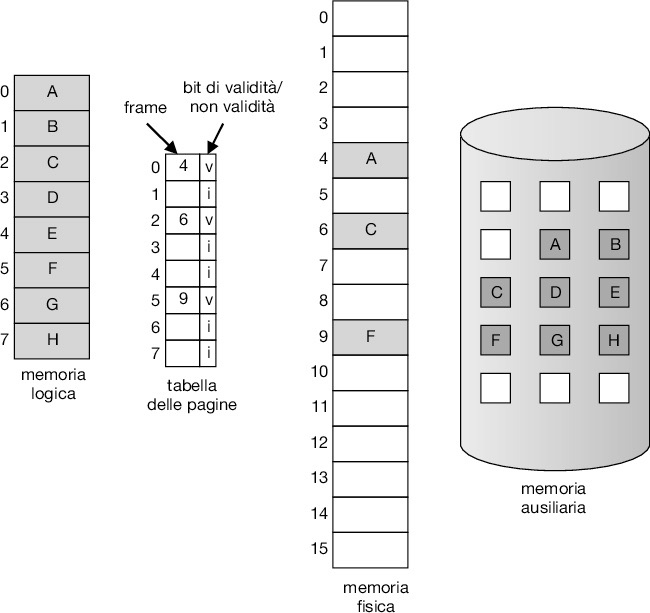
\includegraphics[width=0.25\linewidth]{images/table_of_pages_notAllInRam.png} \caption{Tabella delle pagine non presente totalmente in RAM} \label{fig:10.4} \end{figure}
\begin{figure}[h] \centering 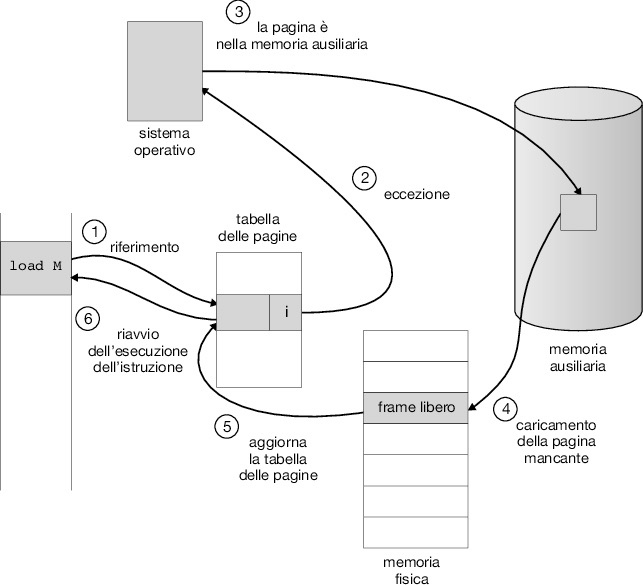
\includegraphics[width=0.25\linewidth]{images/page_fault_gestion.png} \caption{Gestione del Page Fault} \label{fig:10.5} \end{figure}

\section{Demand Paging}
\nt{
    Un processo può essere avviato senza che alcuna delle sue pagine sia inizialmente in Memoria Primaria (MP). Alla prima istruzione indirizzata dal Program Counter (PC), inizializzato dal Sistema Operativo (SO), si genera un \emph{page fault}, poiché il PC punta a un indirizzo di una pagina del processo non presente in MP. Questo schema è chiamato \emph{Pure Demand Paging}.
}

In alternativa, il SO può caricare preventivamente in MP almeno la pagina contenente la prima istruzione da eseguire.

\section*{Supporto Hardware per la Memoria Virtuale}

\nt{
    Per implementare la memoria virtuale è necessario un supporto hardware specifico:
    \begin{itemize}
        \item La tabella delle pagine deve includere un \emph{bit di validità} che l’hardware può testare per generare il \emph{page fault}.
        \item Le istruzioni devono essere ri-eseguibili in caso di \emph{page fault} oppure, alternativamente, l’hardware della CPU deve controllare la presenza in MP di tutti gli operandi prima di eseguire l'istruzione.
    \end{itemize}
}

\nt{
    Sebbene la paginazione possa essere aggiunta a qualsiasi sistema, la \emph{paginazione su richiesta} e, più in generale, la \emph{memoria virtuale}, richiedono un supporto hardware specifico.
}

\section*{Tempo di Accesso Effettivo}

Supponiamo di dover leggere un dato in MP:
\begin{itemize}
    \item \emph{ma} = tempo di accesso in MP se il dato è presente (es. 100-200 nanosecondi)
    \item \emph{p} = probabilità di un page fault
    \item \emph{eat} (effective access time) = 
    \[
    \text{eat} = [(1 - p) \times ma] + [p \times \text{tempo di gestione del page fault}]
    \]
\end{itemize}

\clm{Passi per la gestione di un page fault}{}{
    L’elenco completo dei passi necessari a gestire un page fault è descritto nel testo, ma le tre operazioni principali sono:
    \begin{enumerate}
        \item \textbf{Gestione del page fault}: richiede da 1 a 100 μsec.
        \item \textbf{Recupero della pagina mancante dalla Memoria Secondaria (MS)}: circa 8 millisecondi. Questo valore può variare a seconda del sistema, ma, se la memoria secondaria è su Hard Disk, l’ordine di grandezza è comunque di qualche millisecondo.
        \item \textbf{Riavvio del processo}: richiede da 1 a 100 μsec.
    \end{enumerate}
    \nt{I tempi per i punti 1 e 3 sono trascurabili rispetto al punto 2.}
}

\section*{Calcolo del Tempo di Accesso Effettivo}

Assumendo \textit{ma} = 200 nanosecondi, otteniamo (valori espressi in nanosecondi):
\[
\text{eat} = (1 - p) \times 200 + p \times 8.000.000 = 200 + p \times 7.999.800
\]

\ex{Calcolo con probabilità di page fault}{ 
    Se consideriamo \( p = 0.001 \) (un page fault ogni 1000 accessi), allora:
    \[
    \text{eat} = 200 + 0.001 \times 7.999.800 = 8.199,8 \text{ (circa 8,2 microsecondi)}
    \]
    \nt{In questo caso, l’esecuzione rallenta di oltre 40 volte!}
}

\qs{Degrado massimo del 10\%}{
    Per avere un degrado massimo del 10\%, la probabilità \( p \) deve rispettare la seguente disuguaglianza:
    \[
    \text{eat} = 220 > 200 + 8 \times 10^6 \times p
    \]
    \[
    20 > 8 \times 10^6 \times p
    \]
    \[
    p < 2,5 \times 10^{-6}
    \]
    Questo significa che non ci dovrebbero essere più di un page fault ogni 400.000 accessi in memoria.
}

\qs{400.000 accessi: sono molti o pochi?}{
    Se un processo esegue circa un milione di istruzioni, quanti accessi in RAM genera approssimativamente?
    \nt {
        1 milione di istruzioni = 1 milione di accessi in RAM (ogni istruzione richiede almeno un accesso in RAM).
        Alcune istruzioni possono richiedere più accessi in RAM, ma 1 milione è un buon punto di partenza.
    }
}

\nt{
    Il numero di page fault deve essere estremamente basso per evitare un aumento inaccettabile del tempo medio di esecuzione dei processi. Se il numero di page fault è elevato, il \textit{throughput} del sistema peggiora invece di migliorare.
}

\nt{
    È possibile intervenire anche sul tempo di gestione del page fault. Ad esempio:
    \begin{itemize}
        \item Usare pagine di grandi dimensioni, che possono ridurre il numero medio di page fault. (Perché?);
        \item Ottimizzare l'accesso alla Memoria Secondaria, anche se questa strategia presenta limiti, poiché implica comunque l’uso di hard disk. Si veda anche il capitolo 11, che tratta delle memorie a stato solido.
    \end{itemize}
}


\subsection{L'area di swap}


\dfn{Memoria Virtuale e Area di Swap}{
    Per funzionare, la memoria virtuale necessita di una porzione dedicata dell'Hard Disk, detta \textit{area di swap}.
}

\nt{
    Al momento dell'installazione del sistema operativo (SO), viene riservata una porzione del disco come area di swap ad uso esclusivo del SO. Questa area è gestita con meccanismi più semplici ed efficienti rispetto a quelli del file system:
    \begin{itemize}
        \item Le pagine dei processi non vengono salvate all'interno di file, evitando così l'uso dei file descriptor;
        \item Spesso, vengono utilizzati blocchi più grandi, con allocazione contigua, per migliorare le prestazioni di accesso (questo concetto sarà più chiaro nella parte sulla gestione della memoria secondaria).
    \end{itemize}
}

\clm{Utilizzo dell'Area di Swap}{}{
    Un modo semplice di usare l'area di swap consiste nel copiare l'eseguibile intero di un processo nell'area di swap all'avvio del processo:
    \begin{itemize}
        \item Il tempo di avvio del processo aumenta;
        \item Sono necessarie aree di swap di grandi dimensioni;
        \item Tuttavia, la gestione dei page fault è più veloce, poiché il recupero delle pagine è più rapido una volta che queste sono già nell'area di swap, senza passare attraverso il file system.
    \end{itemize}
}

\clm{Uso Alternativo dell'Area di Swap}{}{
    In alternativa, le pagine dell’eseguibile o di eventuali file di dati possono essere lette direttamente dal file system:
    \begin{itemize}
        \item Utile quando occorre limitare le dimensioni dell'area di swap;
        \item L’avvio dei processi è più veloce;
        \item L'esecuzione può risultare più lenta rispetto all'uso della swap.
    \end{itemize}
}

Notiamo che l’area di swap sembra meno utile se viene utilizzata solo per ospitare gli eseguibili e gli eventuali dati in input prima di avviare i processi. 
Funzione Principale dell'Area di Swap
L’area di swap viene utilizzata soprattutto per:
\begin{itemize}
    \item Liberare spazio in memoria primaria (MP) per ospitare pagine mancanti, caricate in RAM in risposta a un page fault.
\end{itemize}


\nt{
    In effetti, se ci fosse sempre un frame libero, una pagina verrebbe caricata in MP solo la prima volta che viene indirizzata. Tuttavia, l'idea principale della memoria virtuale è di:
    \begin{itemize}
        \item Permettere l'esecuzione di un processo più grande della memoria primaria disponibile.
        \item Consentire l'esecuzione simultanea di processi che, nel complesso, richiedono più spazio di quello disponibile in RAM.
    \end{itemize}
}

Si consideri la situazione in cui due processi occupano più spazio di quello disponibile in memoria principale (cfr. Fig. 10.9).
\begin{figure}[h] \centering 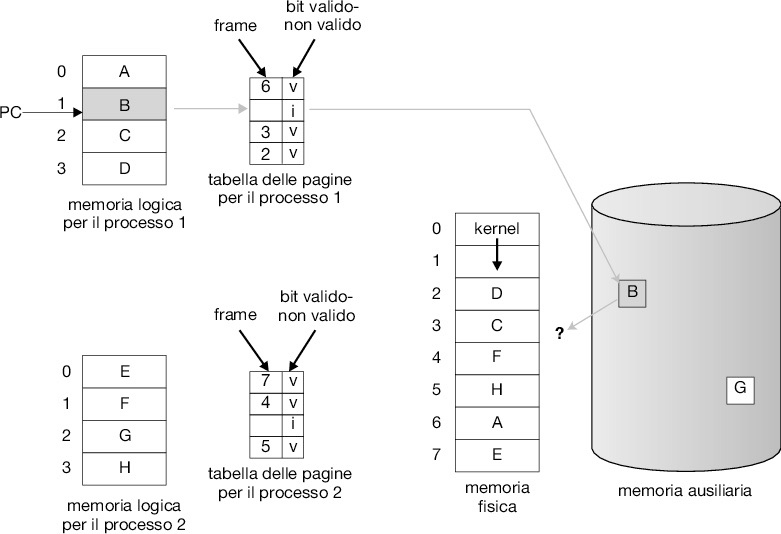
\includegraphics[width=0.5\linewidth]{images/swap_disegno.png} \caption{Swap 10.9} \label{fig:10.9} \end{figure}
Dunque, se si verifica un page fault e tutti i frame della RAM sono occupati, occorre liberarne uno rimuovendo la
agina che ospita, che prende il nome di \textbf{pagina vittima}.\\
Se la pagina vittima contiene dati modificati o fa parte dello stack o della heap di un processo, la pagina va salvata nell’area di swap, in modo che possa essere recuperata quando il processo a cui appartiene vi farà riferimento.\\
Le pagine di codice non devono essere salvate, tanto ce n’è comunque una copia nel file system, ma se erano state copiate inizialmente nell’area di swap potranno poi essere recuperate più velocemente se riferite di nuovo.\\


\section{Sostituzione delle pagine}
\qs{Cosa succede se si verifica un page fault e non c'è alcun frame libero in RAM?}{
    In questo caso, il sistema operativo esegue i seguenti passi:
    \begin{itemize}
        \item Seleziona una pagina "vittima" da rimuovere.
        \item Salva la pagina vittima nell'area di swap (se necessario).
        \item Carica la pagina mancante nel frame liberato.
    \end{itemize}
}

\nt{
Questa procedura è simile al concetto di \textit{swapping} di processi interi. Tuttavia, con la memoria virtuale, il sistema sposta tra RAM e hard disk solo frammenti di processo, ossia una pagina alla volta.
}

\nt{
Se la pagina vittima non è stata modificata da quando è stata caricata in RAM, si può evitare di salvarla nuovamente su disco, poiché ne esiste già una copia in memoria secondaria.
}

Se la pagina vittima è stata modificata, il tempo di gestione del page fault raddoppia poiché è necessario sia salvarla che caricare la nuova pagina. Un \textit{dirty bit} associato a ciascuna entry della tabella delle pagine (PT) può semplificare il processo: il \textit{dirty bit} viene settato a 1 dall’hardware della CPU la prima volta che la pagina viene modificata in RAM. In questo modo, solo le pagine vittima con il \textit{dirty bit} a 1 devono essere salvate in memoria secondaria.

\clm{Modifica e salvataggio delle pagine in memoria virtuale}{}{
    Solo le pagine di dati (stack e heap) possono essere modificate e, quindi, avere il \textit{dirty bit} a 1. Le pagine di codice, essendo accedute solo in lettura, non necessitano di essere salvate nell'area di swap se scelte come pagine vittima. Inoltre, se il codice era stato inizialmente copiato nell'area di swap, riportare le pagine di codice in RAM è più rapido rispetto al caricamento dall'eseguibile nel file system.
}

\nt{
La gestione della sostituzione delle pagine è fondamentale per consentire l'esecuzione di programmi più grandi della memoria primaria disponibile. Tuttavia, ciò comporta due problemi rilevanti:
\begin{itemize}
    \item \textbf{Scelta della pagina da sostituire}: Quale pagina scegliere come vittima?
    \item \textbf{Allocazione dei frame}: Quanti frame assegnare a ciascun processo? (aspetto che verrà discusso in seguito)
\end{itemize}
Il metodo utilizzato per risolvere questi problemi influisce notevolmente sulle prestazioni di esecuzione dei processi.
}

\begin{figure}[h] \centering 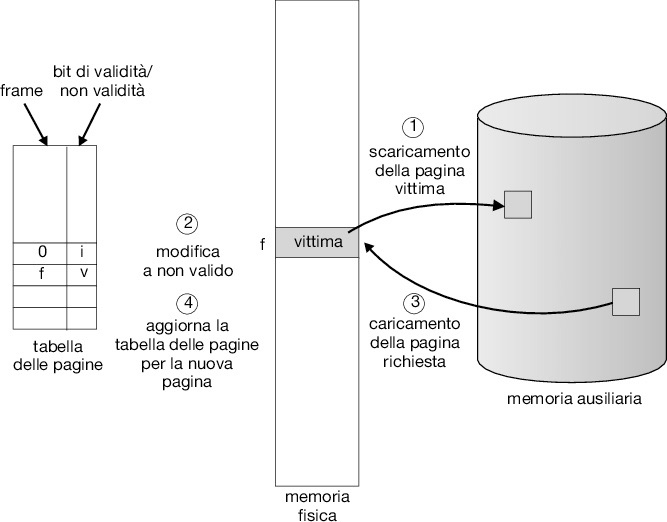
\includegraphics[width=0.50\linewidth]{images/sostituzione_di_pagina.png} \caption{Sostituzione di pagina} \label{fig:10.10} \end{figure}

\subsection{Algoritmi di sostituzione delle pagine}
Se una pagina vittima appena rimossa viene nuovamente indirizzata dal processo a cui appartiene, si verifica un \textit{page fault} e la pagina deve essere ricaricata in memoria principale. In questo caso, parte del lavoro viene sprecato.\\
Al contrario, se la pagina vittima scelta non verrà mai più utilizzata, non sarà necessario ricaricarla in memoria, ottimizzando l'uso della memoria primaria.\\

\clm{Obiettivo degli algoritmi di sostituzione delle pagine}{}{
    Un buon algoritmo di sostituzione minimizza il numero di \textit{page fault}. In letteratura, questi algoritmi sono spesso chiamati \textit{algoritmi di rimpiazzamento delle pagine}.
}

\qs{Come possiamo valutare l'efficacia di diversi algoritmi di sostituzione delle pagine?}{
    Si può valutare l'efficacia tramite sequenze di riferimenti in memoria principale:
    \begin{itemize}
        \item \textbf{generate casualmente}, oppure
        \item \textbf{generate dall'esecuzione di programmi reali}.
    \end{itemize}
    Non interessa l’indirizzo esatto dell'istruzione, ma solo il numero della pagina indirizzata, ignorando quindi l’offset.
}

\ex{Esempio di sequenza di riferimento}{
    Supponiamo che la sequenza di riferimento sia:
    \[
    10, 7, 4, 5, 6, 1, 10, 4, \dots
    \]
    Durante l’esecuzione, la CPU ha generato una sequenza di indirizzi logici che indirizzano le pagine in quest'ordine.
}

\qs{Quanti \textit{page fault} genera questa sequenza di riferimento?}{
    Supponiamo di avere a disposizione un solo frame in memoria. Con questa ipotesi, la sequenza provoca 8 \textit{page fault}.
    
    Consideriamo invece la seguente sequenza:
    \[
    10, 7, 7, 7, 4, 5, 5, 5, 5, 6, 1, 10, 10, 10, 10, 4
    \]
    Anche questa sequenza causa 8 \textit{page fault}, poiché i riferimenti consecutivi alla stessa pagina non generano nuovi \textit{page fault} dopo che la pagina è stata caricata in memoria primaria.
}

\nt{
Pertanto, le sequenze:
\[
10, 7, 4, 5, 6, 1, 10, 4
\]
e
\[
10, 7, 7, 7, 4, 5, 5, 5, 5, 6, 1, 10, 10, 10, 10, 4
\]
sono equivalenti per quanto riguarda la valutazione della bontà di un algoritmo di sostituzione.
}

\nt{
Il numero di \textit{page fault} generati da una sequenza per un dato algoritmo di sostituzione dipende anche dal numero di frame disponibili. Intuitivamente, all’aumentare dei frame disponibili, il numero di \textit{page fault} tende a ridursi — ma come vedremo, ciò non accade sempre!
}
\begin{figure}[h] \centering 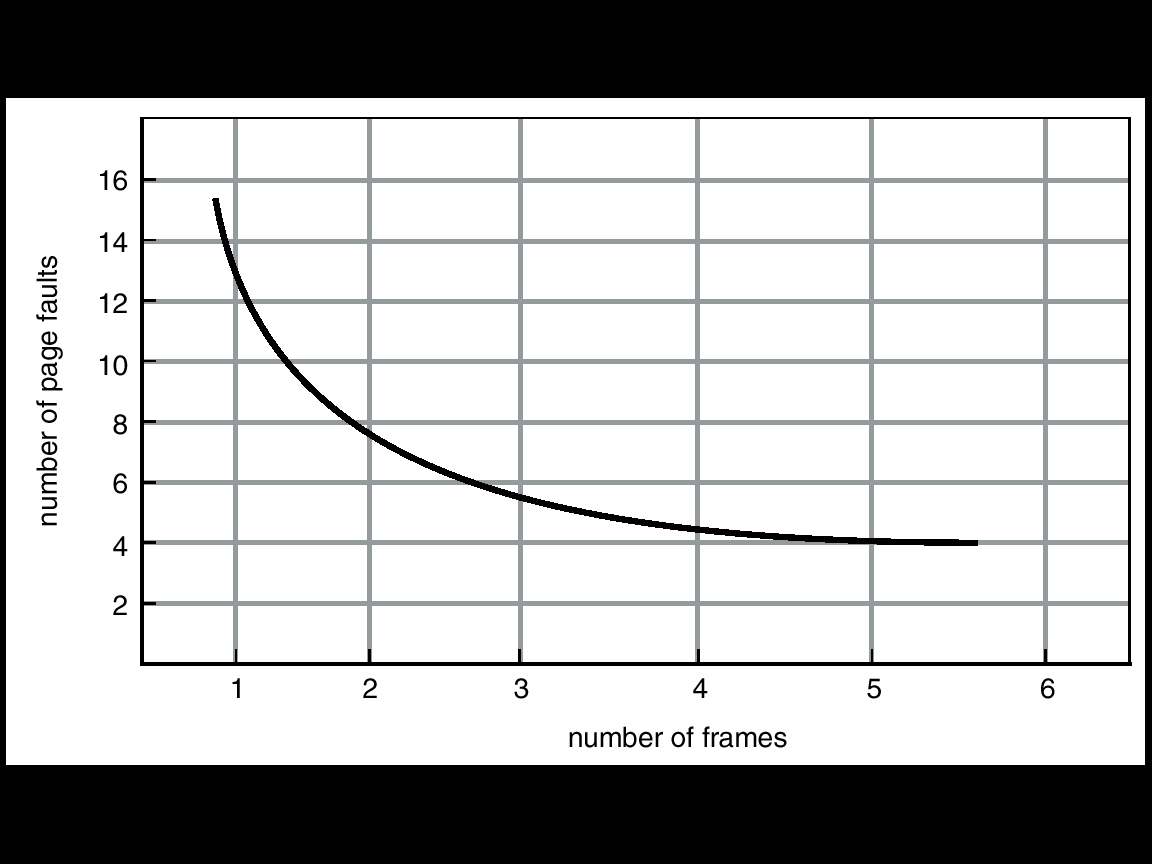
\includegraphics[width=0.50\linewidth]{images/page_faultGraph.png} \caption{Grafico dei page fault} \label{fig:5.4} \end{figure}

\subsection{Sostituzione delle pagine secondo l’ordine d’arrivo (FIFO)}
Nel seguito, assumeremo che a ogni processo venga assegnato un numero prestabilito di frame e che la scelta della pagina vittima avvenga esclusivamente tra le pagine del processo stesso. Questa politica prende il nome di sostituzione \textbf{locale} delle pagine.\\
Assumiamo inoltre uno schema di \textit{paginazione su richiesta puro}: quando un processo inizia, nessuna delle sue pagine è in RAM, e quindi il primo riferimento a una pagina qualsiasi genera un \textit{page fault}.\\

\dfn{Algoritmo FIFO}{
    L’algoritmo \textbf{FIFO} (First In, First Out) sceglie come pagina vittima quella presente da più tempo in memoria principale. Questo approccio è semplice da implementare ma non garantisce sempre buone prestazioni:
    \begin{itemize}
        \item Se la pagina vittima contiene codice di inizializzazione usato solo all'inizio, allora la rimozione va bene, poiché la pagina non verrà più utilizzata.
        \item Tuttavia, se la pagina contiene una variabile usata per tutta l’esecuzione del codice o una procedura richiamata frequentemente, la rimozione potrebbe rivelarsi inefficiente.
    \end{itemize}
}

\ex{Esempio di FIFO}{
    Consideriamo la sequenza di riferimenti:
    \[
    7, 0, 1, 2, 0, 3, 0, 4, 2, 3, 0, 3, 2, 1, 2, 0, 1, 7, 0, 1
    \]
    Con 3 frame disponibili, questa sequenza produce 15 \textit{page fault} (vedi Fig. 10.12).
}
\begin{figure}[h] \centering 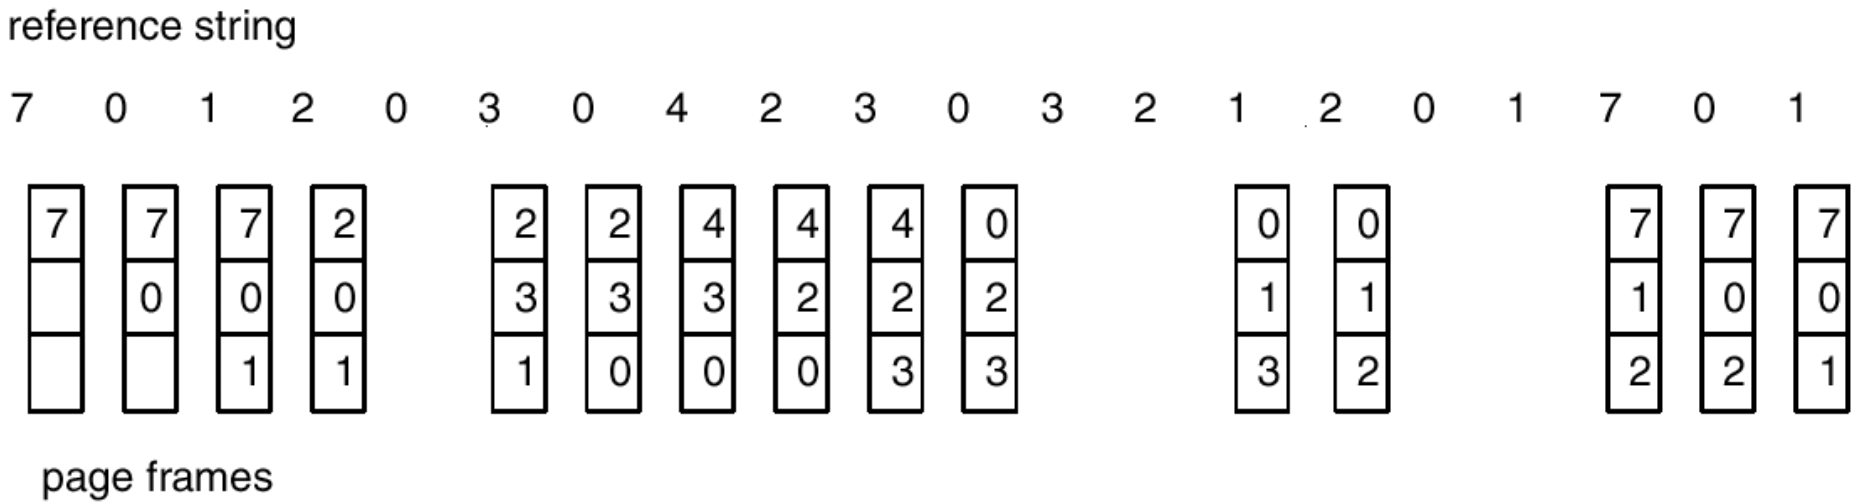
\includegraphics[width=0.50\linewidth]{images/fifo_page_fault.png} \caption{10.12} \label{fig:10.12} \end{figure}

\nt{
L'algoritmo FIFO è affetto dalla cosiddetta \textit{Anomalia di Belady}: in alcuni casi, aumentando il numero di frame, il numero di \textit{page fault} può paradossalmente aumentare!
}

\ex{Anomalia di Belady}{
    Consideriamo la seguente stringa di riferimento:
    \[
    1, 2, 3, 4, 1, 2, 5, 1, 2, 3, 4, 5
    \]
    In alcuni casi, aumentando il numero di frame, il numero di \textit{page fault} prodotti può aumentare (vedi Fig. 10.13). È importante notare che questo fenomeno si verifica solo per alcune specifiche sequenze di riferimento.
}

\begin{figure}[h] \centering 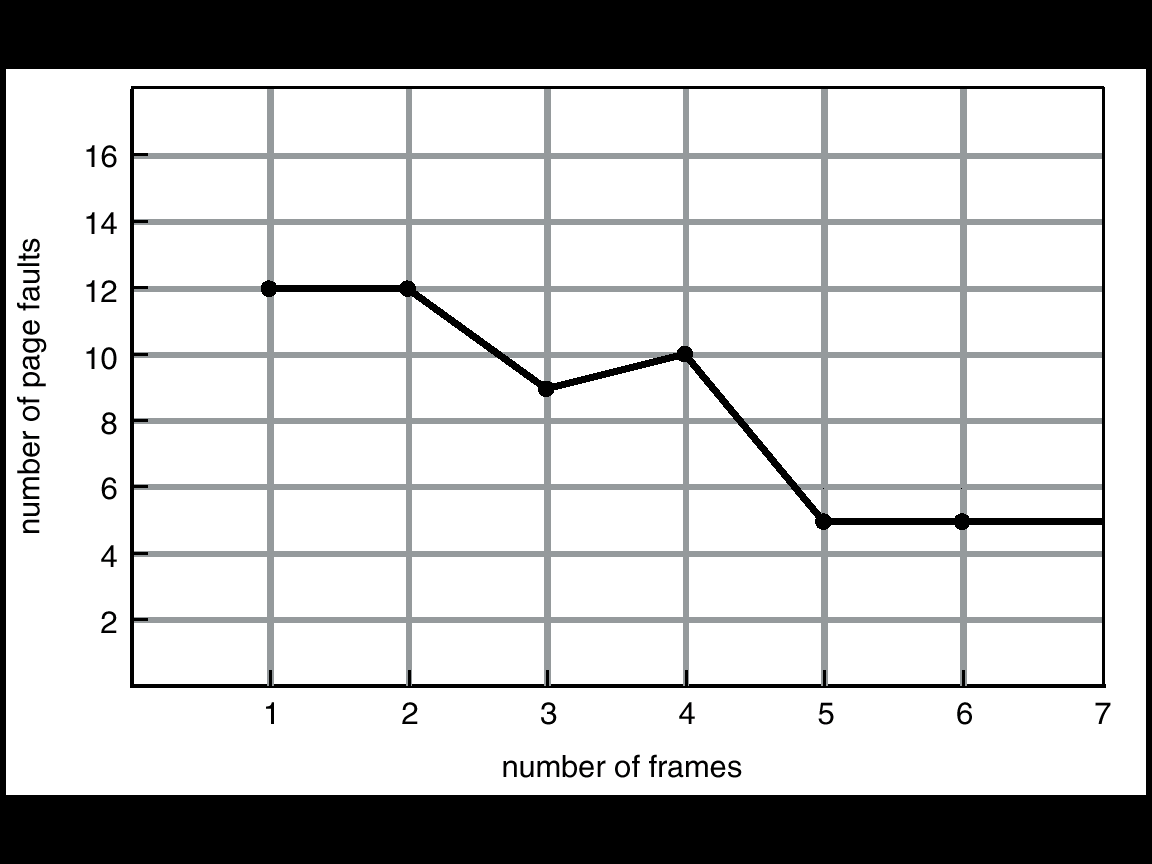
\includegraphics[width=0.33\linewidth]{images/belady_anomaly.png} \caption{10.13} \label{fig:10.13} \end{figure}

\dfn{Algoritmo OPT (o MIN)}{
    L’algoritmo \textbf{OPT}, o \textbf{MIN}, seleziona come vittima la pagina che verrà utilizzata più avanti nel tempo rispetto a tutte le altre pagine attualmente in memoria. Questo algoritmo garantisce il numero minimo di \textit{page fault} per un dato numero di frame, evitando l'anomalia di Belady.
    
    Tuttavia, \textbf{OPT non è implementabile} in un sistema reale, poiché richiederebbe una conoscenza anticipata dell’uso delle pagine. Viene usato solo come termine di paragone per valutare le prestazioni di altri algoritmi.
}

\ex{Esempio di OPT}{
    Utilizzando l'algoritmo OPT con 3 frame, la sequenza:
    \[
    7, 0, 1, 2, 0, 3, 0, 4, 2, 3, 0, 3, 2, 1, 2, 0, 1, 7, 0, 1
    \]
    produce 9 \textit{page fault} (vedi Fig. 10.14).
}

\subsection{Algoritmo LRU (Least Recently Used)}
\nt{
L’algoritmo OPT è ideale perché sceglie come pagina vittima quella che non verrà più utilizzata nel futuro, ma ovviamente non è implementabile. Un tentativo di approssimazione di questo comportamento è l’algoritmo \textbf{LRU} (Least Recently Used), che seleziona come vittima la pagina che non è stata usata da più tempo.
}

\dfn{Algoritmo LRU}{
    L'algoritmo \textbf{LRU} non soffre dell'anomalia di Belady e si avvicina molto a OPT, ma ha il difetto di essere difficile da implementare in modo efficiente. In pratica, LRU guarda al passato (anziché al futuro) per determinare quale pagina rimuovere. Questo approccio funziona bene nella maggior parte dei casi, ma è più complesso da implementare.
}

\ex{Esempio di LRU}{
    Consideriamo la seguente sequenza di riferimenti:
    \[
    7, 0, 1, 2, 0, 3, 0, 4, 2, 3, 0, 3, 2, 1, 2, 0, 1, 7, 0, 1
    \]
    Con 3 frame disponibili, l'algoritmo LRU produce 12 \textit{page fault} (vedi Fig. 10.15).
}
\begin{figure}[h] \centering 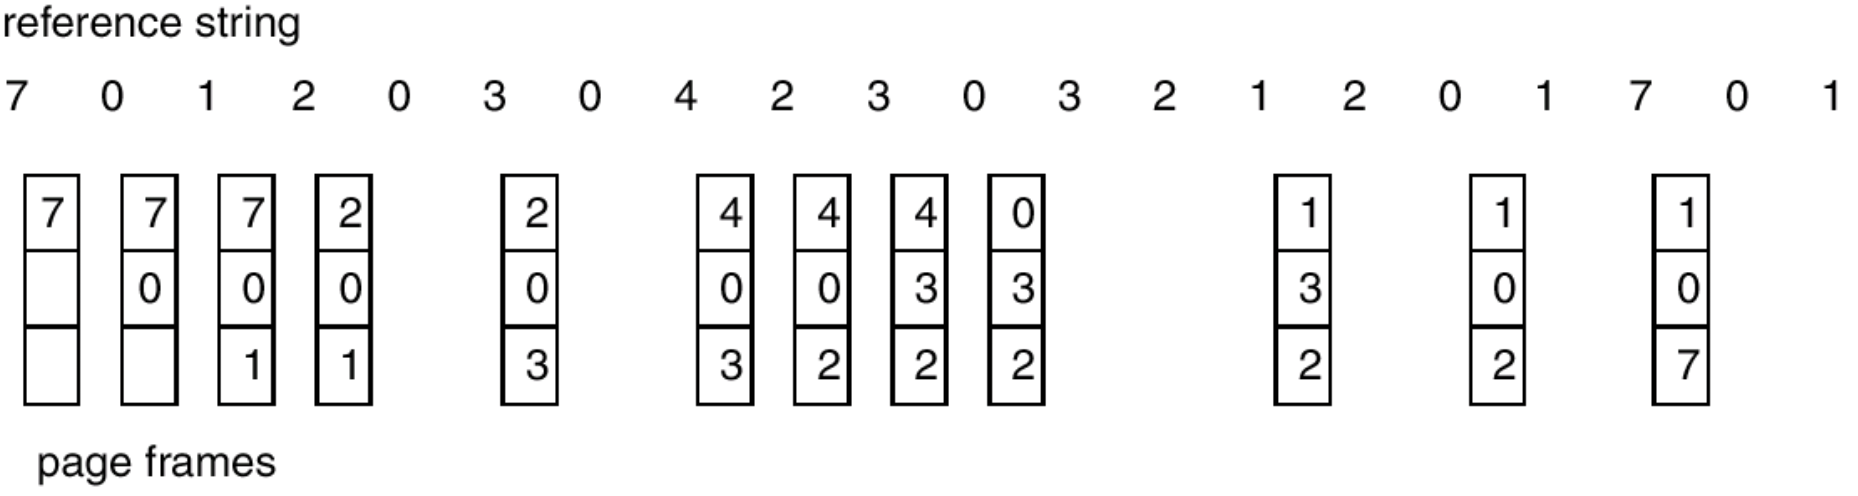
\includegraphics[width=0.50\linewidth]{images/lru_pages_alg.png} \caption{10.15} \label{fig:10.15} \end{figure}
L’implementazione dell'algoritmo LRU richiederebbe un supporto hardware da parte della CPU che, purtroppo, non è disponibile nelle architetture moderne. Tuttavia, esistono approcci che utilizzano un supporto hardware più semplice per approssimare LRU in modo accettabile.

\dfn{Reference Bit}{
    Molti processori forniscono un \textit{reference bit}, un bit associato a ciascuna pagina nella Page Table di un processo. Quando un processo inizia, tutti i reference bit delle sue pagine sono inizializzati a 0 dal sistema. 
    \begin{itemize}
        \item Quando una pagina viene indirizzata (sia in lettura che in scrittura), l'hardware imposta a 1 il reference bit di quella pagina.
        \item In questo modo, possiamo sapere quali pagine sono state utilizzate di recente, anche se non sappiamo l'ordine esatto di accesso.
    \end{itemize}
}

\subsubsection{Algoritmo LRU Seconda Chance}
Partendo da un algoritmo FIFO, in caso di \textit{page fault} il sistema operativo esamina la pagina che è entrata per prima in RAM. Se il reference bit di questa pagina è 0, essa viene scelta come pagina vittima. Se invece il reference bit è 1, la pagina riceve una "seconda chance": il suo reference bit viene azzerato e viene trattata come se fosse appena entrata in memoria.

\dfn{Algoritmo della Seconda Chance}{
    L'algoritmo della seconda chance funziona come segue:
    \begin{itemize}
        \item Se il reference bit di una pagina è 0, la pagina viene selezionata come vittima.
        \item Se il reference bit è 1, il bit viene azzerato e la pagina viene spostata in fondo alla coda FIFO.
    \end{itemize}
    Se in una sequenza di sostituzioni tutte le pagine hanno il reference bit impostato a 1, l'algoritmo riprende a esaminare la prima pagina della coda (quella entrata per prima in RAM) e la seleziona come vittima, tornando di fatto a un algoritmo FIFO.
}
Se una pagina viene riferita frequentemente, il suo reference bit rimarrà a 1 per la maggior parte del tempo, riducendo la probabilità che venga selezionata come vittima. Questo algoritmo è una buona approssimazione di LRU ed è decisamente più efficiente di una gestione completa di LRU in hardware.\\
Se “next victim” non viene riferita prima di una seconda chiamata dell’algoritmo, il suo reference bit resta a 0, quindi non è stata riferita di recente, e diviene quindi una buona candidata alla sostituzione.\\

\begin{figure}[h] \centering 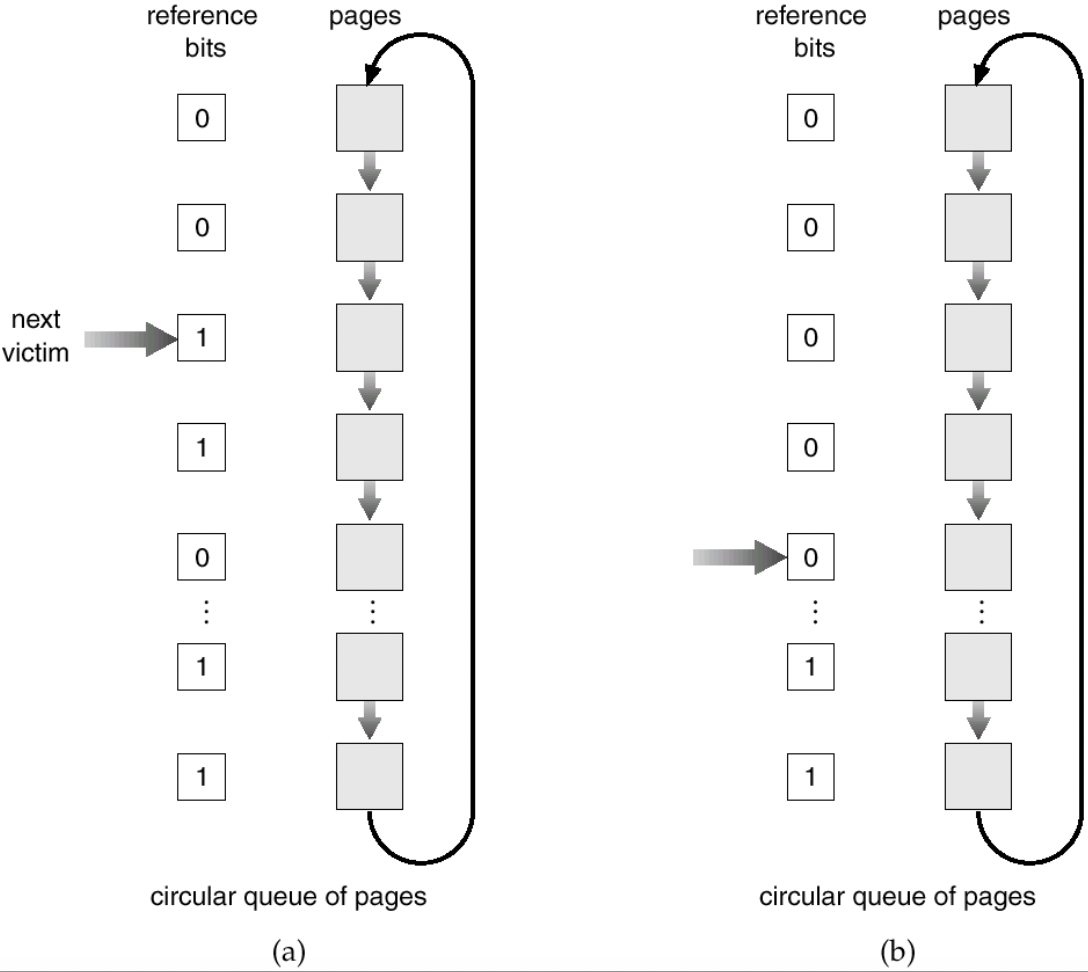
\includegraphics[width=0.25\linewidth]{images/second_chanceQueue.png} \caption{10.17} \label{fig:10.17} \end{figure}

\subsection{Algoritmo Seconda Chance con Dirty Bit} 
Quando l'hardware fornisce sia il \textit{reference bit} che il \textit{dirty bit}, le pagine possono essere classificate in quattro gruppi, ognuno dei quali ha una priorità diversa per essere sostituito:

\dfn{Classificazione delle Pagine}{
    Le pagine sono raggruppate in base a due bit: il \textit{reference bit} e il \textit{dirty bit}.
    \begin{itemize}
        \item \textbf{(0, 0)}: La pagina non è stata utilizzata di recente e non è stata modificata. È la migliore da rimpiazzare.
        \item \textbf{(1, 0)}: La pagina è stata utilizzata di recente, ma non è stata modificata. È una buona candidata, ma meno preferibile rispetto a quella (0, 0).
        \item \textbf{(0, 1)}: La pagina non è stata utilizzata di recente, ma è stata modificata. È meno buona da sostituire, in quanto dovrà essere salvata in memoria secondaria per non perdere le modifiche.
        \item \textbf{(1, 1)}: La pagina è stata utilizzata di recente e modificata. È la peggiore da sostituire, poiché richiede di essere salvata in memoria secondaria prima di essere rimossa.
    \end{itemize}
}
Il principio di sostituzione applicato in questo algoritmo è simile a quello della "Seconda Chance". In questo caso, si seleziona come vittima la prima pagina che appartiene alla classe migliore non vuota (quella con il valore \textbf{(0, 0)} se disponibile, poi \textbf{(1, 0)}, e così via).

\dfn{Algoritmo di Sostituzione con Reference e Dirty Bit}{
    L'algoritmo, che si basa su questa classificazione delle pagine, è utilizzato in molti sistemi operativi Unix e in macOS. La scelta della pagina da rimpiazzare dipende dallo stato combinato dei bit di riferimento e di modifica, con la preferenza per le pagine meno utilizzate e non modificate.
}

\section{Allocazione dei Frame}
In un sistema multiprogrammato, la distribuzione dei frame disponibili tra i processi può essere gestita in vari modi:

\dfn{Strategie di Distribuzione dei Frame}{
    \begin{itemize}
        \item \textbf{Allocazione uniforme}: Ogni processo riceve lo stesso numero di frame. Ad esempio, se ci sono $n$ frame e $p$ processi, ogni processo ottiene $n/p$ frame.
        \item \textbf{Allocazione proporzionale}: I frame vengono distribuiti in base alle dimensioni di ogni processo. Ad esempio, se i processi sono di dimensioni diverse, i processi più grandi riceveranno più frame.
        \item \textbf{Allocazione proporzionale in base alla priorità}: La distribuzione dei frame tiene conto della priorità dei processi. I processi con priorità più alta ricevono più frame.
        \item \textbf{Allocazione con riserva di frame}: Alcuni frame devono essere tenuti liberi per consentire l'ingresso di nuovi processi nel sistema.
    \end{itemize}
}

\dfn{Esempio di Allocazione Proporzionale}{
    Se abbiamo 11 frame disponibili e i processi P1, P2 e P3 hanno dimensioni rispettive di 4, 6 e 12 pagine, la distribuzione dei frame sarà:
    \begin{itemize}
        \item P1: 2 frame,
        \item P2: 3 frame,
        \item P3: 6 frame.
    \end{itemize}
}
Nel caso dell'allocazione proporzionale in base alla priorità, il numero di frame assegnati a ciascun processo dipenderà dalla priorità relativa dei processi (e in alcuni casi dalle loro dimensioni).\\

\dfn{Allocazione dei Frame e Grado di Multiprogrammazione}{
    \nt{
    Qualunque schema di allocazione venga scelto, il numero di frame assegnato a ciascun processo cambierà in funzione del grado di multiprogrammazione. 
    }
}

\dfn{Strategie di Selezione della Vittima per la Rimozione}{
    In caso di page fault, bisogna scegliere quale pagina rimuovere dalla memoria principale:
    \begin{itemize}
        \item \textbf{Allocazione globale}: La vittima è scelta fra tutte le pagine in memoria principale, esclusi i frame utilizzati dal sistema operativo. Questo approccio potrebbe rimuovere una pagina di un altro processo rispetto a quello che ha causato il page fault.
        \item \textbf{Allocazione locale}: La vittima è scelta fra le pagine del processo che ha causato il page fault, mantenendo costante il numero di frame allocato a ciascun processo.
    \end{itemize}
}

\wc{Problemi}{
\textbf{Problemi dell'Allocazione Globale}: La strategia globale rende il turnaround di un processo fortemente dipendente dal comportamento degli altri processi, con un elevato rischio di variazione nelle prestazioni da un'esecuzione all'altra. 

\textbf{Problemi dell'Allocazione Locale}: Se un processo riceve troppi frame, ciò può ridurre il throughput complessivo del sistema, poiché gli altri processi avranno meno frame disponibili e genereranno più page fault.
}

\nt {
Si è visto sperimentalmente che l’allocazione globale fornisce in genere un throughput maggiore e riesce a gestire la multiprogrammazione in maniera più flessibile.\\
L’allocazione globale è di solito preferita per sistemi time sharing, in cui molti utenti possono usare contemporaneamente il sistema.\\
I sistemi Windows usano l’allocazione locale, mentre Linux e Solaris usano l’allocazione globale delle pagine.\\
}

\subsection{Thrashing (attività di paginazione degenere)}
\nt{
Consideriamo un sistema in cui, in un dato momento, ogni processo ha a disposizione un numero ridotto di frame, cioè ogni processo ha in memoria principale (MP) un numero di pagine inferiore rispetto al numero totale di pagine di cui è composto. Supponiamo anche di adottare una allocazione globale dei frame. Va sottolineato che il problema del \textbf{thrashing} si può verificare anche nel caso di allocazione locale dei frame. 
}

\dfn{Probabilità di Page Fault}{
    Con poche pagine in RAM per processo, la probabilità che ogni processo generi un page fault è alta. In seguito a un page fault, una pagina vittima viene rimossa dalla memoria principale (MP), probabilmente da un altro processo. 

    Questo altro processo, a sua volta, avrà ancora meno pagine in memoria, aumentando ulteriormente la probabilità che anche esso generi un page fault a breve. Si innesca così un circolo vizioso in cui:
    \begin{itemize}
        \item Ogni processo genera continuamente page fault,
        \item I frame vengono "rubati" tra i vari processi,
        \item La probabilità di page fault aumenta continuamente.
    \end{itemize}
}

\dfn{Thrashing}{
    Questo fenomeno è noto come \textbf{thrashing}, che si verifica quando il sistema tenta di aumentare eccessivamente il grado di multiprogrammazione, ossia cercando di eseguire più processi contemporaneamente per sfruttare al massimo la CPU e incrementare il throughput del sistema. 

    Tuttavia, oltre una certa soglia, i processi passano più tempo a gestire i page fault generati che ad eseguire realmente il loro lavoro. Di conseguenza, la \textit{utilizzazione della CPU} diminuisce drasticamente e il \textit{throughput} del sistema crolla. 
}

\dfn{Relazione tra Grado di Multiprogrammazione e Thrashing}{
    Il grado di multiprogrammazione è direttamente legato al rischio di thrashing. Aumentando il numero di processi che cercano di essere eseguiti contemporaneamente, cresce anche la probabilità che ognuno di essi abbia pochi frame disponibili. Questo può portare a una situazione in cui il sistema è sopraffatto dalla gestione dei page fault, riducendo di fatto l'efficienza complessiva. 

    La relazione tra grado di multiprogrammazione e throughput diventa inversamente proporzionale oltre una certa soglia, con l'aumento della multiprogrammazione che inizialmente porta a un miglioramento delle prestazioni, ma che successivamente provoca un forte degrado delle stesse a causa del thrashing.
}

\begin{figure}[h] \centering 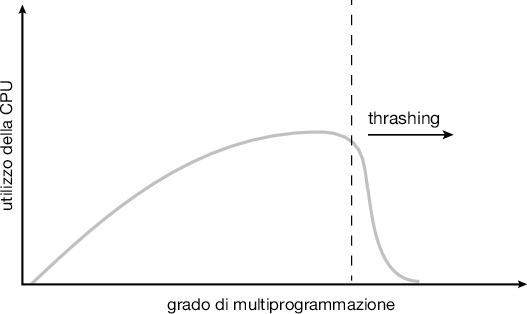
\includegraphics[width=0.55\linewidth]{images/tharsing_multiporgGraph.png} \caption{10.20} \label{fig:10.20} \end{figure}

\subsection{Cause del Thrashing}
Se il livello di utilizzo della CPU di un sistema è troppo basso, lo si può alzare aumentando in grado di permettendo a più utenti di connettersi, e/o di lanciare un maggior numero di processi. In questo modo però, i nuovi processi incominciano a sottrarre pagine ai processi già presenti, per “farsi un po' di spazio”. Fino ad un certo punto l’aumento di processi è ben tollerato dal sistema, poiché ciascun processo ha comunque una quantità sufficiente di frame a disposizione da poter girare senza generare troppi page fault. Ma se si esagera, ci si può avvicinare alla soglia del thrashing: molti processi incominciano a generare dei page fault e, come conseguenza, vengono tolti dalla RQ e messi in una coda di wait in attesa della pagina mancante. Risultato? La RQ si svuota, e il livello di utilizzo della CPU scende. Beh, ma se la CPU è sotto-utilizzata, si può lanciare qualche altro processo, o permettere a qualche altro utente di collegarsi... E la situazione non fa che peggiorare!.\\
Nei moderni sistemi time-sharing, il ciclo perverso è spesso innescato dagli utenti, che lanciano altri programmi senza attendere la fine di quelli già in esecuzione, sperando così di aumentare la percentuale del tempo di CPU globale che riescono ad usare a loro vantaggio.\\
In definitiva quindi, il thrashing è una sorta di “ingolfamento” del sistema: vogliamo sfruttarlo al meglio “iniettando” più e più processi nel sistema, fino ad arrivare ad un punto in cui i processi si ostacolano a vicenda.\\
La soluzione giusta sarebbe di diminuire il grado di multiprogrammazione temporaneamente, in modo che i processi non rimossi dalla MP abbiano il tempo di terminare correttamente prima di far (ri)partire gli altri.\\


\subsection{Come combattere il Thrashing}
In definitiva, quindi, il \textit{thrashing} rappresenta una sorta di “ingolfamento” del sistema: si tenta di sfruttare al massimo le risorse “iniettando” più processi possibili, ma si finisce per raggiungere un punto in cui i processi si ostacolano a vicenda.

\nt{
    La soluzione ottimale consiste nel ridurre temporaneamente il grado di multiprogrammazione. Così facendo, i processi ancora presenti in memoria possono completare correttamente la loro esecuzione, prima di permettere l'avvio (o il riavvio) di altri processi.
}

\clm{Frequenza accettabile dei page fault}{}{
    È possibile stabilire, ad esempio in base ad osservazioni sperimentali, un livello “accettabile” di frequenza di page fault, per raggiungere le prestazioni desiderate:
    \begin{itemize}
        \item \textbf{Se la frequenza osservata è troppo bassa}, si possono rimuovere alcuni frame dai processi e aumentare il grado di multiprogrammazione.
        \item \textbf{Se la frequenza osservata è troppo alta}, occorre diminuire il grado di multiprogrammazione e redistribuire i frame liberati tra i processi ancora attivi.
    \end{itemize}
}

\nt{
    Il \textit{thrashing} può essere prevenuto monitorando attentamente la frequenza dei page fault (come illustrato in figura 10.23).
}

\begin{figure}[h] \centering 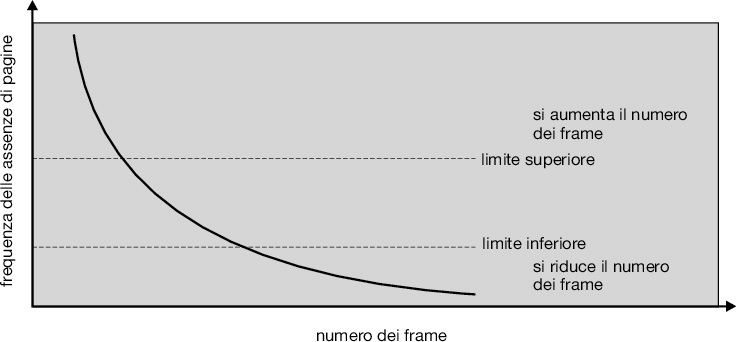
\includegraphics[width=0.50\linewidth]{images/frequenctOfPageFault.png} \caption{Frequenza dei page fault} \label{fig:10.23} \end{figure}

Adottare una politica di sostituzione locale può contribuire a ridurre il rischio di thrashing, poiché i processi non possono sottrarsi le pagine tra loro. Se un singolo processo entra in thrashing, non danneggia gli altri, sebbene possa utilizzare intensivamente le risorse di I/O su disco.

Tuttavia, se si assegnano troppi pochi frame a ciascun processo per aumentare eccessivamente il grado di multiprogrammazione, esiste il rischio che tutti i processi entrino in thrashing.

\cor{Prevenzione ottimale del thrashing}{
    La migliore prevenzione del thrashing è dotare il sistema di una quantità sufficiente di memoria principale.
}

\section{Dimensioni delle pagine}
Sono sempre potenze di $2$; ma quanto dovrebbero essere grandi? 

\begin{itemize}
    \item \textbf{Pagine piccole} implicano:
    \begin{itemize}
        \item Tabelle delle pagine (PT) più grandi;
        \item meno frammentazione interna;
        \item peggiori prestazioni nell’uso dell'HD, poiché il \textit{seek} e la latenza del disco sono costanti (si vedrà meglio nel Capitolo 11);
        \item in generale, un maggior numero di page fault (immaginiamo pagine di un solo byte in pure demand paging).
    \end{itemize}
    
    \item \textbf{Pagine grandi} presentano le considerazioni opposte.
\end{itemize}

A causa della diminuzione del costo della RAM e dell’aumento degli spazi di indirizzamento fisico disponibili, la tendenza è quella di usare pagine sempre più grandi. Negli anni ’80, $4$ Kbyte era considerata la dimensione massima accettabile di una pagina, mentre oggi tale valore è normale, e spesso anche superato. 

\nt{
    L'aumento costante della quantità di RAM nei sistemi moderni ha fatto sì che, nel tempo, il problema del \textit{thrashing} e, più in generale, le problematiche legate alla memoria virtuale abbiano un impatto minore sulle prestazioni complessive dei sistemi.
}

\subsection{Struttura dei programmi}
Il modo in cui i programmi utilizzano i dati influisce significativamente sul numero di page fault generati.

\begin{itemize}
    \item Ad esempio, gli \textbf{array bidimensionali} sono allocati per riga: se scriviamo codice che accede agli elementi per colonna, aumentiamo il rischio di page fault. Supponiamo che una pagina contenga esattamente una riga dell'array; cosa accade se è allocato un solo frame per contenere una parte dell’array?

    \item Le \textbf{tabelle hash} possono offrire prestazioni scarse con la memoria virtuale, poiché anche dati concettualmente contigui vengono memorizzati in modo sparpagliato.
\end{itemize}

Consideriamo l'array bidimensionale:

\[
\texttt{char A[1024][1024];}
\]

Ogni riga è memorizzata in una pagina, e all'array è assegnato un solo frame (di $1024$ byte) in RAM. L’array è memorizzato per righe:
\[
\texttt{A[0][0], A[0][1], A[0][2], \ldots, A[0][1023], A[1][0], \ldots}
\]

\begin{itemize}
    \item \textbf{Programma 1}: 
    \begin{verbatim}
        for (j = 0; j < 1024; j++)
            for (i = 0; i < 1024; i++) A[i][j] = '0';
    \end{verbatim}
    
    \item \textbf{Programma 2}:
    \begin{verbatim}
        for (i = 0; i < 1024; i++)
            for (j = 0; j < 1024; j++) A[i][j] = '0';
    \end{verbatim}
\end{itemize}

\qs{}{
    Quale programma genera meno page fault? E quanti?
    \newline
    Quale programma genera più page fault? E quanti?
}

\nt{
    Il \textbf{Programma 1} genera più fault, perchè accede prima colonna per colonna, $(1024*1024)$ page fault.\\
    Il \textbf{Programma 2} genera meno fault, perchè accede prima riga per riga, $(1024)$ page fault.
}

\section{Gestione nei Sistemi Operativi}
\subsection{Windows}
In Windows 10 viene implementata la \textit{demand paging with clustering}: quando una pagina viene caricata in memoria, vengono caricate anche alcune pagine adiacenti, che si presume possano essere usate a breve.

Alla creazione di un processo, vengono assegnati a quest'ultimo due numeri:
\begin{itemize}
    \item \textbf{Insieme di lavoro minimo}: il numero minimo di pagine che il sistema operativo garantisce di allocare in RAM per quel processo (di solito, 50);
    \item \textbf{Insieme di lavoro massimo}: il numero massimo di pagine che il sistema operativo allocherà in RAM per quel processo (di solito, 345).
\end{itemize}

Il sistema operativo mantiene anche una lista di \textbf{frame liberi}, con un numero minimo di frame da mantenere liberi in lista.

\begin{itemize}
    \item Se un processo $P$ genera un page fault e non ha ancora raggiunto il suo insieme di lavoro massimo, la pagina mancante viene portata in RAM e assegnata a un frame libero.
    \item Se invece $P$ ha raggiunto il suo insieme di lavoro massimo, viene scelta una \textbf{pagina vittima} tra quelle di $P$, quindi viene applicata una politica di sostituzione locale delle pagine.
\end{itemize}

Se il numero di frame liberi in RAM scende al di sotto del limite minimo, viene avviata una procedura per liberare spazio:
\begin{itemize}
    \item Ciascun processo che ha in RAM un numero di pagine superiore al proprio insieme di lavoro minimo vedrà rimosse dalla RAM tutte le pagine in eccesso.
    \item Nei sistemi con processore Intel, per decidere quali pagine rimuovere viene utilizzato l’\textbf{algoritmo della seconda chance}.
\end{itemize}

\subsection{Solaris}
\nt{
    Solaris utilizza una normale \textit{paginazione su richiesta}, assegnando un frame libero in caso di page fault. Un parametro, \texttt{lostfree}, associato all'elenco dei frame liberi e pari di solito a $1/64$ del numero di frame in cui è suddivisa la RAM, indica il numero minimo di frame liberi desiderati.
}

Ogni $1/4$ di secondo, il sistema operativo controlla se il numero di frame liberi è inferiore a \texttt{lostfree}. In tal caso, viene attivato il processo \textbf{pageout}, che funziona in due fasi applicando una variante dell'algoritmo della seconda chance:

\begin{itemize}
    \item \textbf{Prima fase}: \texttt{pageout} scorre tutte le pagine allocate in RAM azzerando il bit di riferimento di ciascuna.
    \item \textbf{Seconda fase}: scorre di nuovo tutte le pagine e quelle con bit di riferimento ancora a $0$ vengono considerate riutilizzabili. Le pagine con \textit{dirty bit} a $1$ vengono salvate prima di essere effettivamente riutilizzate.
\end{itemize}

Se un processo accede a una pagina marcata come "riutilizzabile" e in attesa di essere salvata, la pagina viene semplicemente riassegnata a quel processo.

Il tempo tra le due scansioni effettuate da \texttt{pageout} può variare in base ai parametri del sistema operativo, ma è generalmente dell'ordine di alcuni secondi.

\begin{itemize}
    \item Se \texttt{pageout} non riesce a mantenere la quantità di frame liberi a un livello accettabile (stabilito dai parametri di sistema), potrebbe indicare che si sta verificando il fenomeno del \textbf{thrashing}.
    \item In tal caso, il sistema operativo può decidere di rimuovere tutte le pagine di un processo, scegliendo tra quelli che sono rimasti inattivi per il tempo più lungo.
\end{itemize}
